\documentclass[
	12pt,				% tamanho da fonte
	openright,			% capítulos começam em pág ímpar (insere página vazia caso preciso)
	oneside,			% ou twoside
	a4paper,			% tamanho do papel. 
	% -- opções do pacote babel --
	english,			% idioma adicional para hifenização
	french,				% idioma adicional para hifenização
	spanish,			% idioma adicional para hifenização
	brazil				% o último idioma é o principal do documento
	]{abntex2}

% ---
% PACOTES
% ---

% ---
% Pacotes fundamentais 
% ---
%\usepackage{lmodern}			% Usa a fonte Latin Modern			
\usepackage[T1]{fontenc}		% Selecao de codigos de fonte.
\usepackage[utf8]{inputenc}		% Codificacao do documento (conversão automática dos acentos)
%\usepackage{lastpage}			% Usado pela Ficha catalográfica
\usepackage{indentfirst}		% Indenta o primeiro parágrafo de cada seção.
\usepackage{color}				% Controle das cores
\usepackage{graphicx}			% Inclusão de gráficos e figuras
\graphicspath{{figuras/}} %pasta de destino onde estão as figuras
%\usepackage{microtype} 			% para melhorias de justificação
% ---
		
% ---
% Pacotes adicionais, usados apenas no âmbito do Modelo Canônico do abnteX2
% ---
%\usepackage{lipsum}				% para geração de dummy text
% ---

% ---
% Pacotes de citações
% ---
\usepackage[brazilian,hyperpageref]{backref}	 % Paginas com as citações na bibl
\usepackage[alf]{abntex2cite}	% Citações padrão ABNT


% ---
% Informações de dados para CAPA e FOLHA DE ROSTO
% ---
\titulo{Bibliografia de graduação}
\autor{Joan Francisco Alvarez Burgos}
\local{Brasil}
\data{Agosto de 2013}
\orientador{Google Books}
\coorientador{\abnTeX}
\instituicao{%
  Universidade do Estado de Santa Catarina -- UDESC
  \par
  Universidade Federal de Santa Catarina -- UFSC
  }
\tipotrabalho{Trabalho Acadêmico}
% O preambulo deve conter o tipo do trabalho, o objetivo, 
% o nome da instituição e a área de concentração 
\preambulo{Revisão bibliográfica em conformidade às normas da ABNT apresentada à comunidade acadêmica de Engenharia Elétrica sob licença Ceatrive Commons.}
% ---


% ---
% Configurações de aparência do PDF final

% alterando o aspecto da cor azul
\definecolor{blue}{RGB}{41,5,195}

% informações do PDF
\makeatletter
\hypersetup{
     	%pagebackref=true,
		pdftitle={\@title}, 
		pdfauthor={\@author},
    	pdfsubject={\imprimirpreambulo},
	    pdfcreator={LaTeX with abnTeX2},
		pdfkeywords={abnt}{latex}{abntex}{abntex2}{trabalho acadêmico}, 
		colorlinks=true,       		% false: boxed links; true: colored links
    	linkcolor=blue,          	% color of internal links
    	citecolor=blue,        		% color of links to bibliography
    	filecolor=magenta,      		% color of file links
		urlcolor=blue,
		bookmarksdepth=4
}
\makeatother
% --- 

% --- 
% Espaçamentos entre linhas e parágrafos 
% --- 

% O tamanho do parágrafo é dado por:
\setlength{\parindent}{1.3cm} %Tamanho de tabulacão (indentacão)

% Controle do espaçamento entre um parágrafo e outro:
\setlength{\parskip}{0.2cm}  % tente também \onelineskip

% ---
% compila o indice
% ---
\makeindex
% ---

% ----
% Início do documento
% ----
\begin{document}

% Retira espaço extra obsoleto entre as frases.
\frenchspacing 

% ----------------------------------------------------------
% ELEMENTOS PRÉ-TEXTUAIS
% ----------------------------------------------------------
% \pretextual

% ---
% Capa e Folha de Rosto
% ---
\imprimircapa
\imprimirfolhaderosto*
% ---

% ---
% Dedicatória
% ---
\begin{dedicatoria}
   \vspace*{\fill}
   \centering
   \noindent
   \textit{ Este trabalho é dedicado ...} \vspace*{\fill}
\end{dedicatoria}
% ---

% ---------------------------------------------------
% Agradecimentos
% ---------------------------------------------------
\begin{agradecimentos}
Obrigado

\end{agradecimentos}
% ---

% ---------------------------------------------------
% Epígrafe
% ---------------------------------------------------
%\epigraph{\textit{"John Coffey, the electricity shall now be passed through your body until you are dead, in	according with state law. May god have mercy on your soul..."}}{Paul Edgecomb in Green Mile Film}
\begin{epigrafe}
    \vspace*{\fill}
	\begin{flushright}
		\textit{``John Coffey, the electricity shall now be passed \\
		trrough your body until you are dead, in according\\
		with state law. May god have mercy on your soul..."\\
		(Paul Edfecomb in Green Mile Film)}
	\end{flushright}
\end{epigrafe}
% ---

% ---------------------------------------------------
% RESUMOS
% ---------------------------------------------------

% resumo em português
\setlength{\absparsep}{18pt} % ajusta o espaçamento dos parágrafos do resumo
\begin{resumo}
Aqui vai o resumo.

 \textbf{Palavras-chaves}: latex. abntex. editoração de texto.
\end{resumo}

% resumo em inglês
\begin{resumo}[Abstract]
 \begin{otherlanguage*}{english}
   Here it go the Abstract

   \vspace{\onelineskip}
 
   \noindent 
   \textbf{Key-words}: latex. abntex. text editoration.
 \end{otherlanguage*}
\end{resumo}

% resumo em espanhol
\begin{resumo}[Resumen]
 \begin{otherlanguage*}{spanish}
   El resumen carepoto.
  
   \textbf{Palabras clave}: latex. abntex. publicación de textos.
 \end{otherlanguage*}
\end{resumo}
% ---

% ---------------------------------------------------
% inserir lista de ilustrações
% ---------------------------------------------------
%\pdfbookmark[0]{\listfigurename}{lof}
\listoffigures*
\cleardoublepage
% ---

% ---------------------------------------------------
% inserir lista de tabelas
% ---------------------------------------------------
%\pdfbookmark[0]{\listtablename}{lot}
\listoftables*
\cleardoublepage
% ---

% ---------------------------------------------------
% inserir lista de abreviaturas e siglas
% ---------------------------------------------------
\begin{siglas}
  \item[Fig.] Area of the $i^{th}$ component
\end{siglas}
% ---

% ---------------------------------------------------
% inserir lista de símbolos
% ---------------------------------------------------
\begin{simbolos}
  \item[$ \Gamma $] Letra grega Gama
\end{simbolos}
% ---

% ---------------------------------------------------
% inserir o sumario
% ---------------------------------------------------
%\pdfbookmark[0]{\contentsname}{toc}
\tableofcontents*
\cleardoublepage
% ---



% ----------------------------------------------------------
% ELEMENTOS TEXTUAIS
% ----------------------------------------------------------
\textual

% ----------------------------------------------------------
% Introdução
% ----------------------------------------------------------
\chapter*[Introdução]{Introdução} %o asterisco exclui a numeração e retira do sumário
\addcontentsline{toc}{chapter}{Introdução} %este volta a adicionar ao sumário a introdução
O presente trabalho apresenta uma revisão bibliográfica dos livros utilizados pelo autor durante a sua graduação em engenharia elétrica iniciada na UDESC\footnote{Universidade do Estado de Santa Catarina} e continuada pela UFSC\footnote{Universidade Federal de Santa Catarina}. Estruturada de maneira a ser dividido os semestres por capítulo, e as disciplinas consideradas essenciais em seções. São omitidas disciplinas que apenas foram utilizadas notas de aula durante o progresso da disciplina.\par
A motivação do trabalho surgiu do sentimento de ter algum guia de referências para disciplinas onde o material utilizado era deficitário para o entendimento do conteúdo onde apenas uma nota de aula não era suficiente para aquele que busca não apenas aprender\footnote{a.pren.der: [De \textit{apreender}] \textit{vtd}. 1. Tomar conhecimento de. 2. Tonar-se capaz de (algo), graças a estudo, observação, experiência, etc. 3. Tomar conhecimento de algo, retê-lo na memória, graças a
estudo, observação, experiência, etc. (Dicionário Aurélio)}, mas apreender\footnote{a.pre.en.der: [Lat. \textit{apprehendere}.] \textit{vtd}. 1. Apropriar-se judicialmente de. 2. Segurar, agarrar 3. Assimilar mentalmente (Dicionário Aurélio)} o conteúdo.\par
Além dos livros, o objetivo do autor foi explorar por primeira vez a ferramenta \LaTeX\ e seu suporte \abnTeX\ como treino “café-com-leite” de um TCC e disponibilizar seu código na mais pura filosofia código aberto ou do inglês \textit{open source initiative}\footnote{em algum lugar do github}.
Sem mais delongas são apresentados a seguir os resultados de alguns anos de estudo do autor do elemento que perturba as mentes inquietas e liberta indivíduos das prisões do fanatismo, da ignorância e da tirania, os livros.

%----------
% Pirmeiro Sesmetre
%----------
\chapter{Primeiro Semestre}\label{cap:1sem}
Este semestre não incluía disciplinas de alta complexidade.
\section{Cálculo Diferencial e Integral I}\label{sec:cdi1}
As referências incluíam uma apostila elaborada pelo DMAT\footnote{Departamento de Matemática} do CCT\footnote{Centro de Ciências Tecnológicas} que buscava
a padronização, pois todos os cursos entre as engenharias e licenciaturas realizavam a
mesma prova. A principal referência era o livro \citeonline{calculoA} dos professores da UFSC como mostrado em \autoref{fig:calculoA} para funções, inequações, limites, derivadas, comportamento da funções e integrais indefinidas.
\begin{figure}[!htb] %here, top, or bottom
	\caption{Capa de Calculo A}
	\centering
	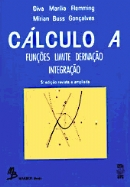
\includegraphics[width=3cm]{calculoA.jpg}
	\legend{Fonte: \citeonline{calculoA}}
	\label{fig:calculoA}
\end{figure}

\section{Geometria Analítica}\label{sec:alg1}
As referências incluíam também uma apostila elaborada pelo DMAT para a introdução de coordenadas polares e utilizava-se o livro \citeonline{geometriaanalitica} da \autoref{fig:geomanalit} para a introduo do R3, retas, planos e as cônicas.
\begin{figure}[!htb]
	\caption{Capa de Geometria Analítica}
	\centering
	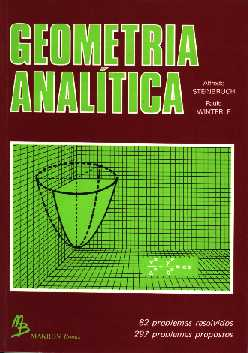
\includegraphics[width=3cm]{geometriaanalitica.jpg}
	\legend{Fonte: \citeonline{geometriaanalitica}}
	\label{fig:geomanalit}
\end{figure}

\chapter{Segundo Semestre}\label{chap:2sem}
Depois de acostumado ao ritmo universitário.
\section{Cálculo Diferencial e Integral II}\label{sec:cdi2}
Já em cálculo II o conteúdo dava sua continuidade com a integrais definidas pela sua definição onde era usado uma apostila elaborada pelo DMAT para este fim e como complemento, o segundo livro de \citeonline{calculoB} como mostrado em \autoref{fig:calculoB} e finalizado pelo estudo de séries como disposto em \citeonline[Cap. 10]{antonseries} mostrado em \autoref{fig:antonseries}.

\begin{figure}[!htb]
	\caption{Capa de Cálculo B}
	\centering
	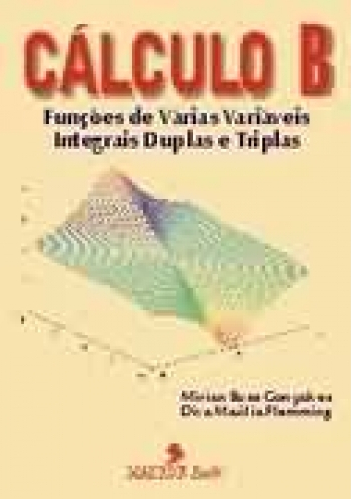
\includegraphics[width=3cm]{calculoB.jpg}
	\legend{Fonte: \citeonline{calculoB}}
	\label{fig:calculoB}
\end{figure}

\begin{figure}[!htb]
	\caption{Capa de Cálculo: um novo horizonte}
	\centering
	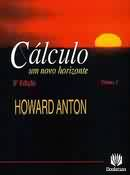
\includegraphics[width=3cm]{antonseries.jpg}
	\legend{Fonte: \citeonline{antonseries}}
	\label{fig:antonseries}
\end{figure}

\section{Algebra Linear}\label{sec:alg2}
O livro de \citeonline{antonalg2} e um livro muito bom em detalhes, porém como a álgebra linear é uma disciplina um tanto que abstrata, o intuito  é servir como introdução para as aplicações em controle moderno que trabalha com equações no domínio do tempo (ou especificamente chamado variáveis de estado) como mostrado mais adiante na \autoref{sec:cmo} e para processamento de sinais que serão especificamente estudadas na área de interesse do aluno. O livro ideal considerado pelo autor para resolver questões relacionadas à matemática é \citeonline{algebralinear} mostrado em \autoref{fig:algebralinear} que vai direto ao ponto.
\begin{figure}[!htb]
	\caption{Capa de Álgebra Linear com Aplicações}
	\centering
	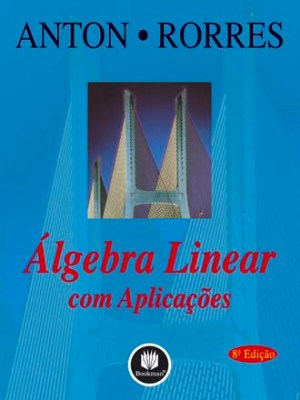
\includegraphics[width=3cm]{antonalg2.jpg}
	\legend{Fonte: \citeonline{antonalg2}}
	\label{fig:antonalg2}
\end{figure}
\begin{figure}[!htb]
	\caption{Capa de Algebra Linear}
	\centering
	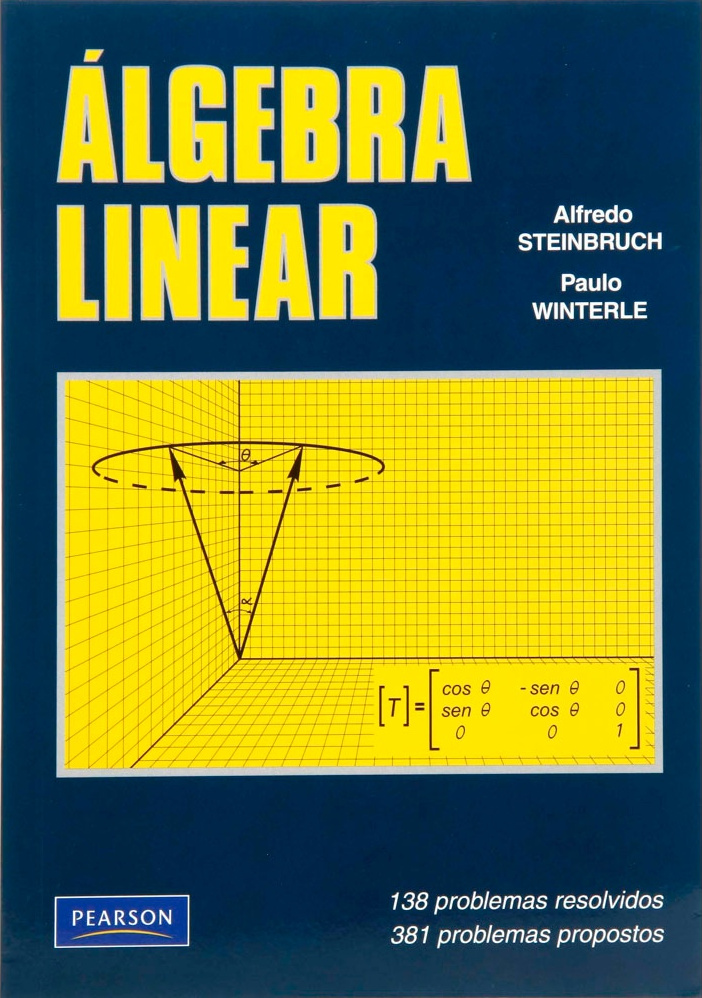
\includegraphics[width=3cm]{algebralinear.jpg}
	\legend{Fonte: \citeonline{algebralinear}}
	\label{fig:algebralinear}
\end{figure}


\section{Fisica Geral I}\label{sec:fge1}
O livro mais utilizado por todo o mundo é o livro da \autoref{fig:halliday1} que possui várias novas edições, porém a usada foi uma versão mais antiga. Ocorre de aparecerem métodos de resolução um tanto que incompreensíveis pelo aluno devido ao fato de haver integração de vetores, porém ao longo do curso, será apenas compreendido mais adiante na \autoref{sec:cve}.

\begin{figure}[!htb]
	\caption{Capa de Física Geral 1}
	\centering
	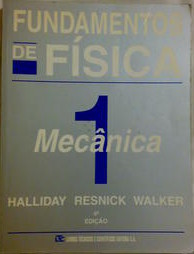
\includegraphics[width=3cm]{halliday1.jpg}
	\legend{Fonte: \citeonline{halliday1}}
	\label{fig:halliday1}
\end{figure}

\section{Química Geral}\label{sec:qge}
A disciplina de Química Geral, apesar de ser muito interessante, não é de caráter imprescindível na visão do autor, apenas de caráter introdutório, para eletrólise e fenômenos tais como a velocidade das reações a qual requer o cálculo diferencial e probabilidade para a região onde pode se encontrar a eletrosfera, como visto nos dois volumes dos livros \citeonline{russel1} e \citeonline{russel2}.

\begin{figure}[!htb]
	\caption{Capa de Química Geral volume 1}
	\centering
	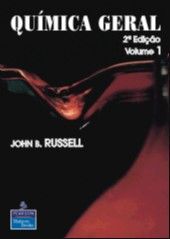
\includegraphics[width=3cm]{russel1.jpg}
	\legend{Fonte: \citeonline{russel1}}
	\label{fig:russel1}
\end{figure}
\begin{figure}[!htb]
	\caption{Capa de Química Geral volume 2}
	\centering
	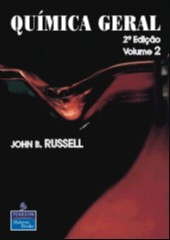
\includegraphics[width=3cm]{russel2.jpg}
	\legend{Fonte: \citeonline{russel2}}
	\label{fig:russel2}
\end{figure}

\chapter{Terceiro Semestre}\label{cap:3sem}
Neste ponto da graduação, é fundamental a compreensão por parte da aluno, pois seu conteúdo requer todo o conhecimento aprendido até aqui e servir de base também para a aprendizagem de praticamente todas as disciplinas do curso com as disciplinas da \autoref{sec:cve} e \autoref{sec:edi}, além de permitir ao aluno a expansão do conhecimento, pelas áreas da mecânica estática, dinâmica, de fluidos e quântica, e de se tratar dos assuntos mais interessantes da física-matemática.

\section{Cálculo Vetorial}\label{sec:cve}
O livro base e mais compreensível considerado pelo autor é o terceiro livro de \citeonline{calculoC} mostrado em \autoref{fig:calculoC} que tem por objetivo apresentar todas as já conhecidas limites, derivadas e integrais, mas na forma vetorial, definir funções escalares e vetoriais e culminar na suas principais ferramentas que facilitaram a compreensão do mundo eletromagnético, os teoremas de Stokes e do grande e todo-poderoso Gauss, ou teorema do rotacional e teorema do divergente respectivamente. Outra referência é o livro para transformação de coordenadas curvilíneas em \citeonline{hsu} que também possui uma boa introdução ao cálculo tensorial\footnote{não visto nesta disciplina}\footnote{O Cálculo Tensorial trata de uma simplificação (complicação para outros) matemática que foi uma evolução além da álgebra cartesiana e álgebra vetorial, através da representação de tensores, sem eles Einstein nunca teria conseguido formular sua teoria geral da relatividade. Melhor explicado em\url{http://www.ime.unicamp.br/~vaz/fismat.htm}}.
\begin{figure}[!htb]
	\caption{Capa de Cálculo C}
	\centering
	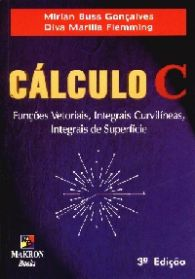
\includegraphics[width=3cm]{calculoC.jpg}
	\legend{Fonte: \citeonline{calculoC}}
	\label{fig:calculoC}
\end{figure}

\section{Equações Diferenciais e Integrais}\label{sec:edi}
Como as equações diferenciais são a forma matemática de representação dos fenômenos físicos, aqui são abordadas as técnicas de resolução e uma boa referência proposta para EDOs\footnote{Equações Diferenciais Ordinárias} é o livro da \autoref{fig:zillcullen1} como introdução e como complemento para resoluções numéricas está o livro da \autoref{fig:zillcullen2}. Agora já para as EDPs\footnote{Equações Diferenciais Parciais} encontra-se o livro antigo, porém útil de \citeonline{kreyszig} que aborda tais resoluções que serão utilizados como método de solução das equações de Laplace e de onda como visto mais adiante na \autoref{sec:emg} e equações de
Schrödinger visto na \autoref{sec:fge6}.
\begin{figure}[!htb]
	\caption{Capa de Equações Diferenciais, volume 1}
	\centering
	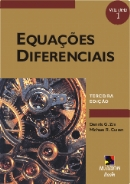
\includegraphics[width=3cm]{zillcullen1.jpg}
	\legend{Fonte: \citeonline{zillcullen1}}
	\label{fig:zillcullen1}
\end{figure}
\begin{figure}[!htb]
	\caption{Capa de Equações Diferenciais, volume 1}
	\centering
	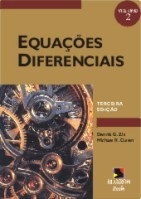
\includegraphics[width=3cm]{zillcullen2.jpg}
	\legend{Fonte: \citeonline{zillcullen2}}
	\label{fig:zillcullen2}
\end{figure}
\begin{figure}[!htb]
	\caption{Capa de Capa de Matemática Superior - Volume 3}
	\centering
	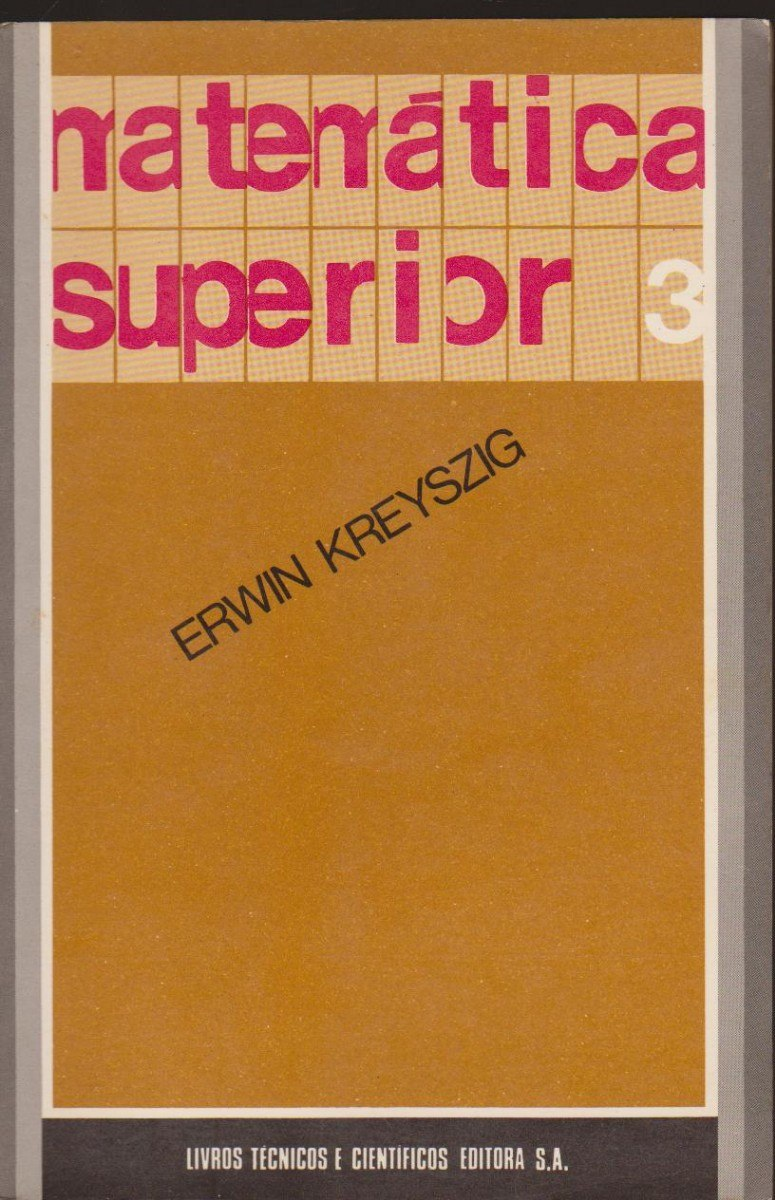
\includegraphics[width=3cm]{kreyszig.jpg}
	\legend{Fonte: \citeonline{kreyszig}}
	\label{fig:kreyszig}
\end{figure}

\section{Física Geral II}\label{sec:fge2}
A disciplina envolve noções básicas de fluidos, termodinâmica, oscilações (movi-
mento harmônico simples) ondas e acústica como visto no livro da \autoref{fig:halliday2}.
\begin{figure}[!htb]
	\caption{Capa de Física Geral 1}
	\centering
	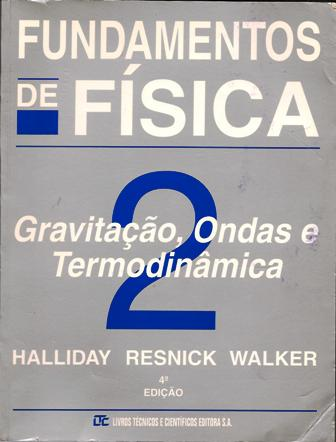
\includegraphics[width=3cm]{halliday2.jpg}
	\legend{Fonte: \citeonline{halliday2}}
	\label{fig:halliday2}
\end{figure}

\section{Mecânica dos Sólidos}\label{sec:mso}
Esta é a primeira noção de uma estrutura real e de como representar um sistema, por seu modelo real, seu modelo físico e modelo matemático do escopo da disciplina que seria uma ponte. Assim foi usando \citeonline{beerjohnston1} que foi visto como calcular forças internas de treliças, vãos de linhas de transmissão e a apresentação da catenária e com \citeonline{popov} o projeto de estruturas submetidas a torções, compressões e trações. Como visto nas \autoref{fig:beerjohnston1} e \autoref{fig:popov}.

\begin{figure}[!htb]
	\caption{Capa de Mecânica Vetorial para Engenheiros}
	\centering
	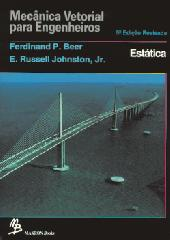
\includegraphics[width=3cm]{beerjohnston1.jpg}
	\legend{Fonte: \citeonline{beerjohnston1}}
	\label{fig:beerjohnston1}
\end{figure}
\begin{figure}[!htb]
	\caption{Capa de Mecânica dos Sólidos}
	\centering
	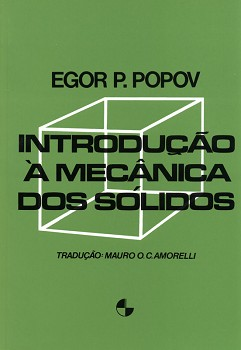
\includegraphics[width=3cm]{popov.jpg}
	\legend{Fonte: \citeonline{popov}}
	\label{fig:popov}
\end{figure}

\section{Processamento de Dados}\label{sec:prd}
A disciplina é introdutória à linguagem de programação. Abordando os conceitos de algoritmo e num primeiro momento a escrita em pseudo-linguagem: portugol para assim entrar no principal assunto que é a linguagem de programação em C, suas ferramentas estruturas e ambientação com o compilador. Utilizado a apostila do professor \citeonline{apostilaUFMG} da UFMG.

\chapter{Quarto Semestre}\label{cap:4sem}
Neste semestre aparecem tópicos avançados tanto da física como da matemática que proporcionam uma ferramenta, mas não um assunto indispensável na visão do autor. Porém é que nos separa das outras engenharias devido à utilização de variáveis complexas à resolução de problemas.

\section{Cálculo Numérico}\label{sec:can}
O escopo da disciplina é aprender a resolver equações quando não é possível se resolver de forma analítica, apresentados os conceitos de interpolação e iteração\footnote{Atenção ao termo iteração, não confundir com interação.}. Usado o livro de \citeonline{calculonumerico} da \autoref{fig:calculonumerico}.

\begin{figure}[!htb]
	\caption{Capa de Cálculo Numérico}
	\centering
	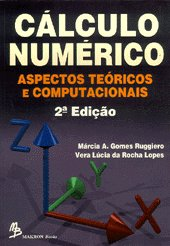
\includegraphics[width=3cm]{calculonumerico.jpg}
	\legend{Fonte: \citeonline{calculonumerico}}
	\label{fig:calculonumerico}
\end{figure}

\section{Cálculo Diferencial e Integral IV}\label{sec:cdi4}
A disciplina é a que introduz os conceitos de funções de uma única variável complexa, polos, zeros e resíduos, assim como o aparecimento de funções especiais que servem como solução de equações diferenciais de alta complexidade que aparecem no eletromagnetismo e na física quântica, apresentados em dois livros na bibliografia a primeira de um autor brasileiro da \autoref{fig:avila} e de outro autor estadunidense da \autoref{fig:churchill}. Culmina na introdução de uma das principais ferramentas dos engenheiros teorizada por Jean-Baptiste Joseph Fourier e tendo em sua homenagem as chamadas Séries de Fourier como apresentado na \autoref{fig:kreyszig}.
\begin{figure}[!htb]
	\caption{Capa de Variáveis Complexas e Aplicações}
	\centering
	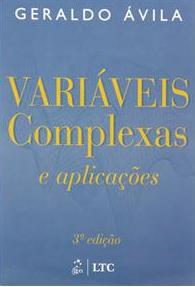
\includegraphics[width=3cm]{avila.jpg}
	\legend{Fonte: \citeonline{avila}}
	\label{fig:avila}
\end{figure}
\begin{figure}[!htb]
	\caption{Capa de Variáveis Complexas e suas Aplicações}
	\centering
	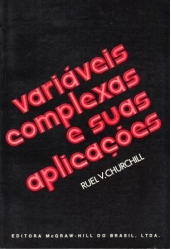
\includegraphics[width=3cm]{churchill.jpg}
	\legend{Fonte: \citeonline{churchill}}
	\label{fig:churchill}
\end{figure}

\section{Física Geral III}\label{sec:fge3}
A disciplina oferece uma abordagem física daquilo relacionado ao mundo eletromagnético. Como uma abordagem introdutória \citeonline{tipler} da \autoref{fig:tipler} oferece uma linguagem de fácil entendimento para um primeiro contato com este assunto. \citeonline{moyses} da \autoref{fig:moyses} apresenta todas as deduções que o eletromagnetismo envolve de forma bem mais profunda e considera-se que é destinado muito mais à física do que à engenharia, já que nas ciências físicas \citeonline{moyses} é o mais referenciado da área. Já \citeonline{sears} da \autoref{fig:sears} apresenta bem o conceito de pressão de radiação. Comparado mais comumente referenciado autor \citeonline{halliday3} existem outros autores como \citeonline{alaorchaves} da \autoref{fig:alaorchaves} que apresentam uma abordagem bem mais teórica de cada tópico que envolve o eletromagnetismo e que apresenta a melhor abordagem daquilo que é o supra-sumo da engenharia elétrica, da disciplina e de tudo que rege nosso universo acadêmico, as oniscientes, onipotentes e onipresentes equações de Maxwell\footnote{James Clerk Maxwell foi responsável por representar matematicamente a relação das grandezas elétricas e magnéticas que anterior à sua publicação eram apenas observadas suas conexões, porém nunca provadas, e.g. na luz os campos elétricos e magnéticos coexistiam em quadratura e a presença e deslocamento tempo-espacial de um campo produz o outro campo de forma recíproca, como será visto mais adiante nos assuntos abordados em \autoref{sec:emg}}.
\begin{figure}[!htb]
	\caption{Capa de Física para cientistas e engenheiros}
	\centering
	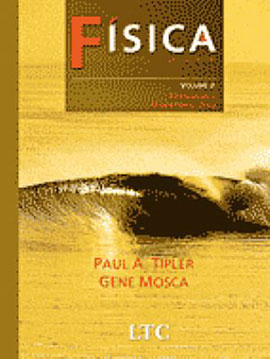
\includegraphics[width=3cm]{tipler.jpg}
	\legend{Fonte: \citeonline{tipler}}
	\label{fig:tipler}
\end{figure}
\begin{figure}[!htb]
	\caption{Capa de Curso de Física Básica: eletromagnetismo}
	\centering
	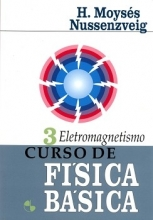
\includegraphics[width=3cm]{moyses.jpg}
	\legend{Fonte: \citeonline{moyses}}
	\label{fig:moyses}
\end{figure}
\begin{figure}[!htb]
	\caption{Capa de Física III: eletromagnetismo}
	\centering
	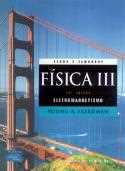
\includegraphics[width=3cm]{sears.jpg}
	\legend{Fonte: \citeonline{sears}}
	\label{fig:sears}
\end{figure}
\begin{figure}[!htb]
	\caption{Capa de Física Básica: Eletromagnetismo}
	\centering
	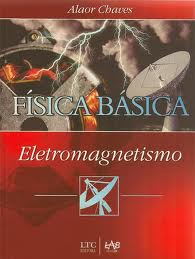
\includegraphics[width=3cm]{alaorchaves.jpg}
	\legend{Fonte: \citeonline{alaorchaves}}
	\label{fig:alaorchaves}
\end{figure}

\chapter{Quinto Semestre}\label{cap:5sem}
Este semestre é a fronteira que separa as disciplinas básicas de engenharia para as disciplinas profissionalizantes.

\section{Estatística}\label{sec:est}

\section{Física Geral IV}\label{sec:fge4}
A disciplina é destinada como introdução à mecânica quântica e seus conceitos preliminares dos comportamentos da onda e da partícula por meio de do livro de \citeonline{feynman} com intuito de apresentar a resolução da Equação de Schrödinger que descreve o estado quântico\footnote{Descrito por uma função de estado, uma função de onda, ou um conjunto de números quânticos.} de um sistema físico usado a principal referência com o livro de \citeonline{eisberg}. Todos estes conceitos são fundamentais para o estudo da radiação visto em Fenômenos de Transporte \autoref{sec:fnt} e principalmente na física do estado sólido, mobilidade dos elétrons,  poços de potencial e junção pn, princípios estes que regem toda a eletrônica vistos em \autoref{sec:ele1}.

\begin{figure}[!htb]
	\caption{Capa de Física em 12 lições}
	\centering
	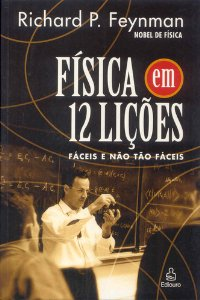
\includegraphics[width=3cm]{feynman.jpg}
	\legend{Fonte: \citeonline{feynman}}
	\label{fig:feynman}
\end{figure}
\begin{figure}[!htb]
	\caption{Capa de Física Quântica}
	\centering
	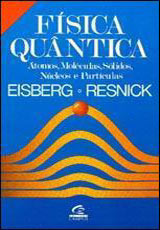
\includegraphics[width=3cm]{eisberg.jpg}
	\legend{Fonte: \citeonline{eisberg}}
	\label{fig:eisberg}
\end{figure}


% ---------------------------------------------------
% Conclusão
% ---------------------------------------------------
%\chapter*[Conclusão]{Conclusão}
%\addcontentsline{toc}{chapter}{Conclusão}



% ----------------------------------------------------------
% Referências bibliográficas
% ----------------------------------------------------------
\bibliography{refsgrad} %aqui vai o nome do arquivo .bib


%---------------------------------------------------------------------
% INDICE REMISSIVO
%---------------------------------------------------------------------

\phantompart
\printindex

\end{document}
